
\documentclass{beamer}

\usepackage[utf8]{inputenc}
\usepackage[spanish]{babel}

\usepackage{beamerthemesplit}

\usetheme{Warsaw}
\usecolortheme{default}

\title{Redes Neuronales Multicapa}
\author{De Santi \and Pereyra \and Pintos }
\subtitle{Sistemas de Inteligencia Artificial}
\date{24 de Abril de 2013}

\AtBeginSection[]
{
  \begin{frame}{Tabla de contenidos}
    \tableofcontents[currentsection]
  \end{frame}
}


\begin{document}

\frame{\titlepage}

\section[Outline]{}
\frame{\tableofcontents}

\section{Introducción}
\subsection{Problema propuesto}
\begin{frame}{Problema propuesto}

\par El problema propuesto fue la estimación de puntos de una serie temporal a partir de una cierta cantidad de puntos anteriores.
\[
  x_{t} = f(x_{t-1}, x_{t-2},...) 
\]

\vspace{10px}
\par No se sabe la cantidad de puntos anteriores a \begin{math} x_{t} \end{math} que se deben tomar para poder estimar.

\end{frame}

\begin{frame}{Gráfico de la serie temporal}

\begin{figure}[H]
\begin{center}
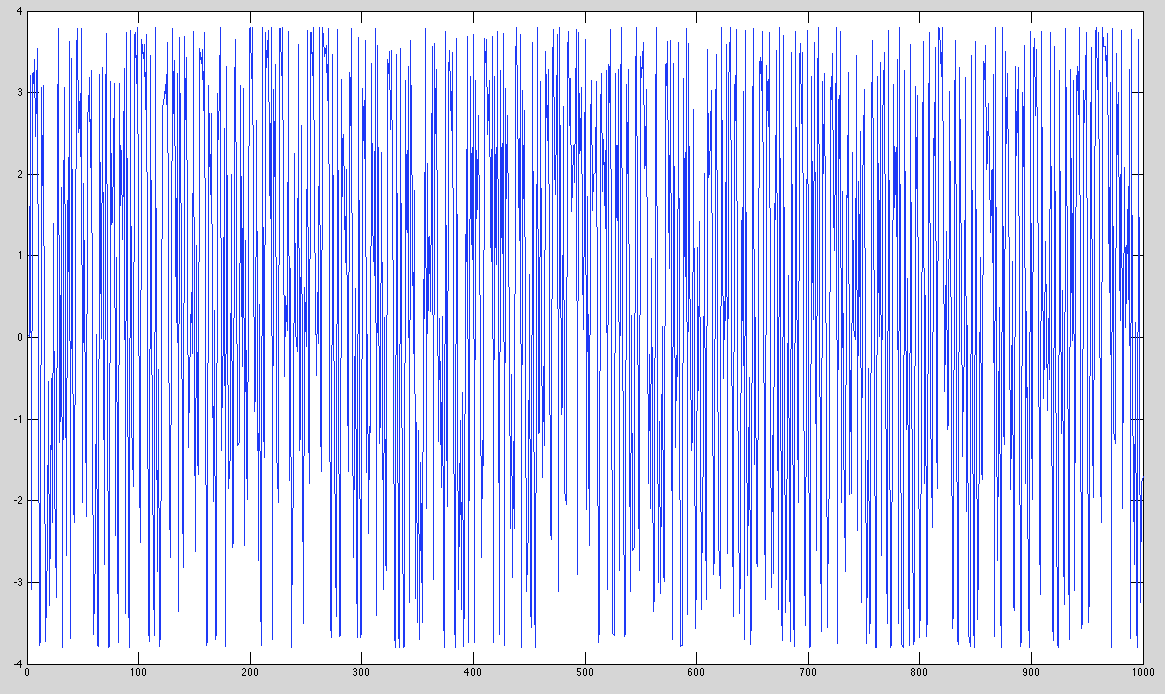
\includegraphics[scale=0.25]{images/serie.png}
\label{modelado}
\end{center}
\end{figure}

\end{frame}




\section{Modelado del problema}
\subsection{Representación de la red neuronal}

\begin{frame}{Representación de la red neuronal}
\par Se representó la red neuronal como una matriz de pesos. \\
\begin{itemize}
\item Cada neurona es una fila de pesos.
\item La matriz tiene tantas filas como neuronas haya en la red.
\end{itemize}
\end{frame}

\subsection{Funciones de activación}
\begin{frame}
\begin{block}{Sigmoidea exponencial}

\[
  f(x) = \frac{2}{1 + e^{-2 \beta x}}  - 1
\]

\[
  f'(x) = 2 \beta \frac{e^{\beta x}}{(e^{\beta x} + 1)^2}
\]

\end{block}

\begin{block}{Tangente hiperbólica}

\[
  f(x) = tanh(\betax) 
\]


\[
  f'(x) = \beta sech(x)^2 
\]

\end{block}

\end{frame}


\subsection{Arquitecturas}

\begin{frame}{¿Qué arquitectura utilizar?}
\par Se probaron diferentes arquitecturas y en base a los resultados se decidió cuál es la mejor arquitectura.
\par Se tuvo en cuenta:
\begin{itemize}
\item Cantidad de capas mínima
\item Cantidad de neuronas mínima
\item ¿Error aceptable en el conjunto de entrenamiento?
\item ¿Error aceptable en el conjunto de testeo?
\end{itemize}
\end{frame}

\subsection{Cálculo del error}

\subsection{Conjuntos de entrenamiento y testeo}
\begin{frame}{Conjunto de entrenamiento y testeo}
\par A partir de los puntos de la serie, se tomo un conjunto al azar para entrenar la red y el resto de los puntos se utilizaron para testear la red entrenada.

\end{frame}

\section{Mejoras al algoritmo backpropagation}

\subsection{Eta adaptativo}
\begin{frame}{$\eta$ adaptativo}
\begin{itemize}
\item Si el error disminuye de manera consistente incrementar $\eta$:
\begin{itemize}
\item ¿Cuánto? 0.1
\item ¿Cuántas veces seguidas se considera consistente? 4 veces

\end{itemize}
\item Si el error incrementa, reducir $\eta$:
\begin{itemize}
\item ¿Cuánto? A la mitad
\end{itemize}
\end{itemize}
\par Estos parámetros afectan al rendimiento de la red!
\end{frame}

\subsection{Momentum}
\begin{frame}{Momentum}
\[w_{ij}(t+1)= - \frac{\partial E}{\partial w{ij}} + \alpha w(t)\]
\par Cambios dependen de cambios anteriores. Idea de dirección general del error. ¿Ayuda un $\alpha$ alto?\\
\par Se pasan todos los patrones, corrigiendo los pesos en cada caso. Una vez pasados, se corrige el eta y se vuelve a comenzar.
\end{frame}

\begin{frame}{Ruido en la derivada de la función de activación}
\par \textbf{Idea:} Escapar de mínimos locales.\\
\par Se le suma un pequeño delta a la derivada para evitar que valga 0 en los mínimos y así poder evitar mínimos locales.
\end{frame}

\section{Resultados}

\begin{frame}{Resultados}
\begin{itemize}
\item Realizamos pruebas exhaustivas en de distintas arquitecturas de red, conjuntos de testeo, combinaciones de momentum y $\eta$ adaptativo. 
\item A continuación mostramos las pruebas más significativas a nuestro criterio.
\end{itemize}
\end{frame}

\begin{frame}{Primera Prueba}
\begin{itemize}
\item Para esta prueba utilizamos un $\eta$ no adaptativo y 500 épocas.
\item El tamaño del conjunto de entrenamiento fue de 400 elementos.
\item Utilizamos una arquitectura de 20 neuronas en una única capa oculta.
\item Obtuvimos un error cuadrático medio de $0.01662$ en el conjunto de entrenamiento.
\item El error cuadrático medio en el conjunto de prueba fue de $0.22923$.
\item Con respecto al conjunto de prueba el $66.33$\% tuvo un error menor a 0.4.
\end{itemize}
\end{frame}
\begin{frame}{Primera Prueba}
\begin{figure}[H]
\begin{center}
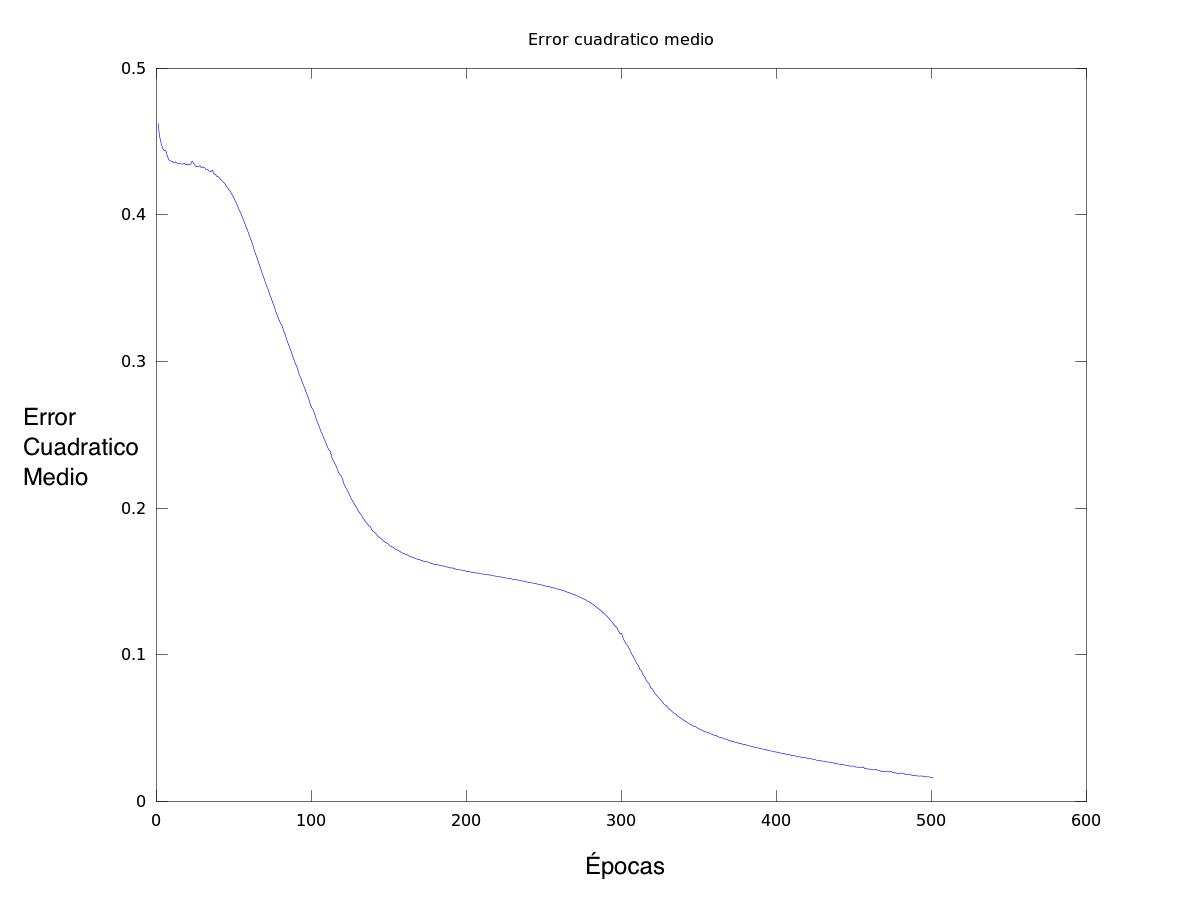
\includegraphics[scale=0.20]{images/t2-4/ecm.png}
\label{modelado}
\end{center}
\end{figure}
\end{frame}

\begin{frame}{Segunda Prueba}
\begin{itemize}
\item Para esta prueba deshabilitamos el momentum probamos por lo cual corrimos 200 épocas.
\item El tamaño del conjunto de entrenamiento fue de 400 elementos.
\item Utilizamos una arquitectura de 9 neuronas en la primera capa oculta, y 6 en la segunda.
\item Obtuvimos un error de $0.00961$ en el conjunto de entrenamiento. 
\item El error cuadrático medio en el conjunto de prueba fue de $0.17816$.
\item Con respecto al conjunto de prueba el $74$\% tuvo un error menor a 0.4.
\end{itemize}
\end{frame}
\begin{frame}{Segunda Prueba}
\begin{figure}[H]
\begin{center}
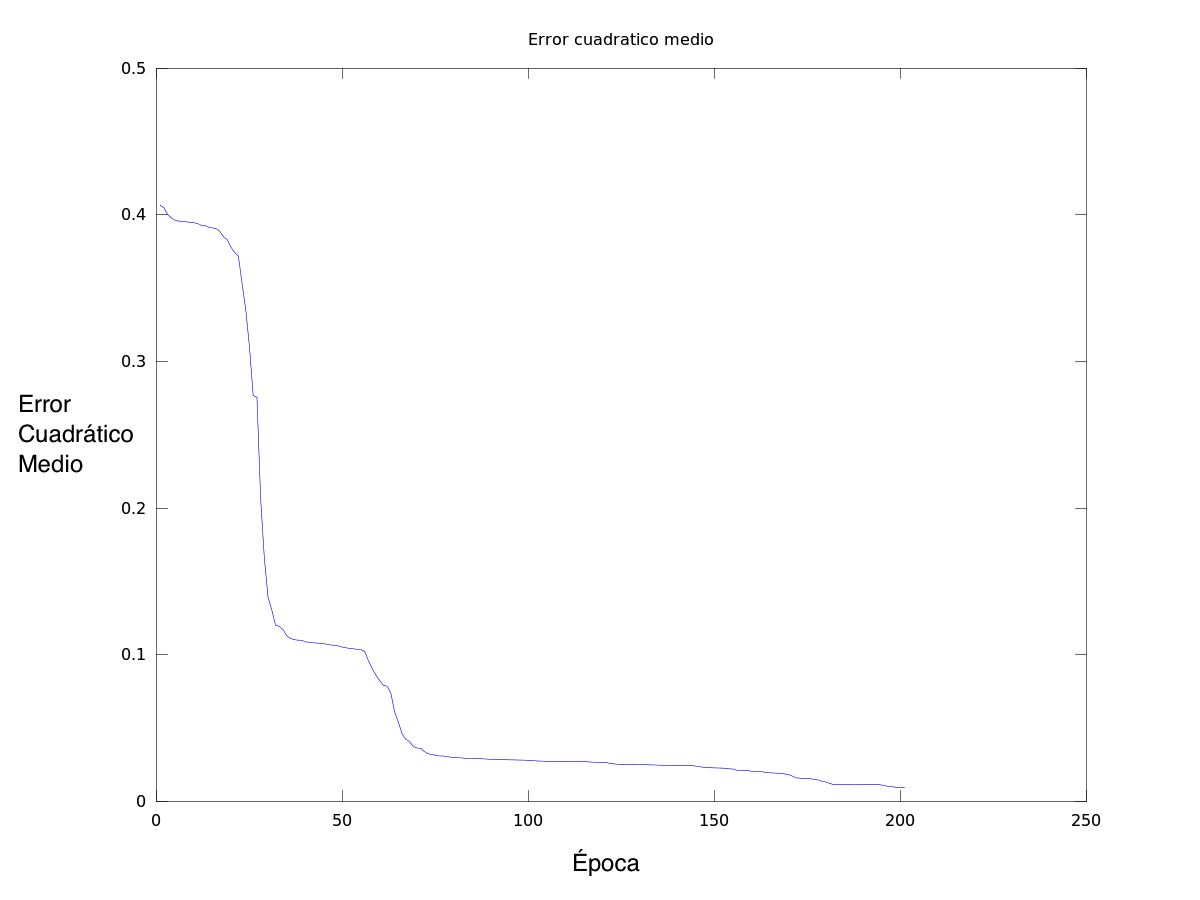
\includegraphics[scale=0.20]{images/t3-10/ecm.png}
\label{modelado}
\end{center}
\end{figure}
\end{frame}

\begin{frame}{Tercera Prueba}
\begin{itemize}
\item Para esta prueba habilitamos tanto momentum como $\eta$ adaptativo.
\item El tamaño del conjunto de entrenamiento fue de 800 elementos.
\item Utilizamos una arquitectura de 9 neuronas en la primera capa oculta, y 6 en la segunda.
\item Obtuvimos un error cuadrático medio de $0.00598$ en el conjunto de entrenamiento. 
\item El error cuadrático medio en el conjunto de prueba fue de $0.07760$.
\item Con respecto al conjunto de prueba el $83$\% tuvo un error menor a 0.4.
\item Fue el mejor resultado en nuestra tanda de pruebas.
\end{itemize}
\end{frame}
\begin{frame}{Tercera Prueba}
\begin{figure}[H]
\begin{center}
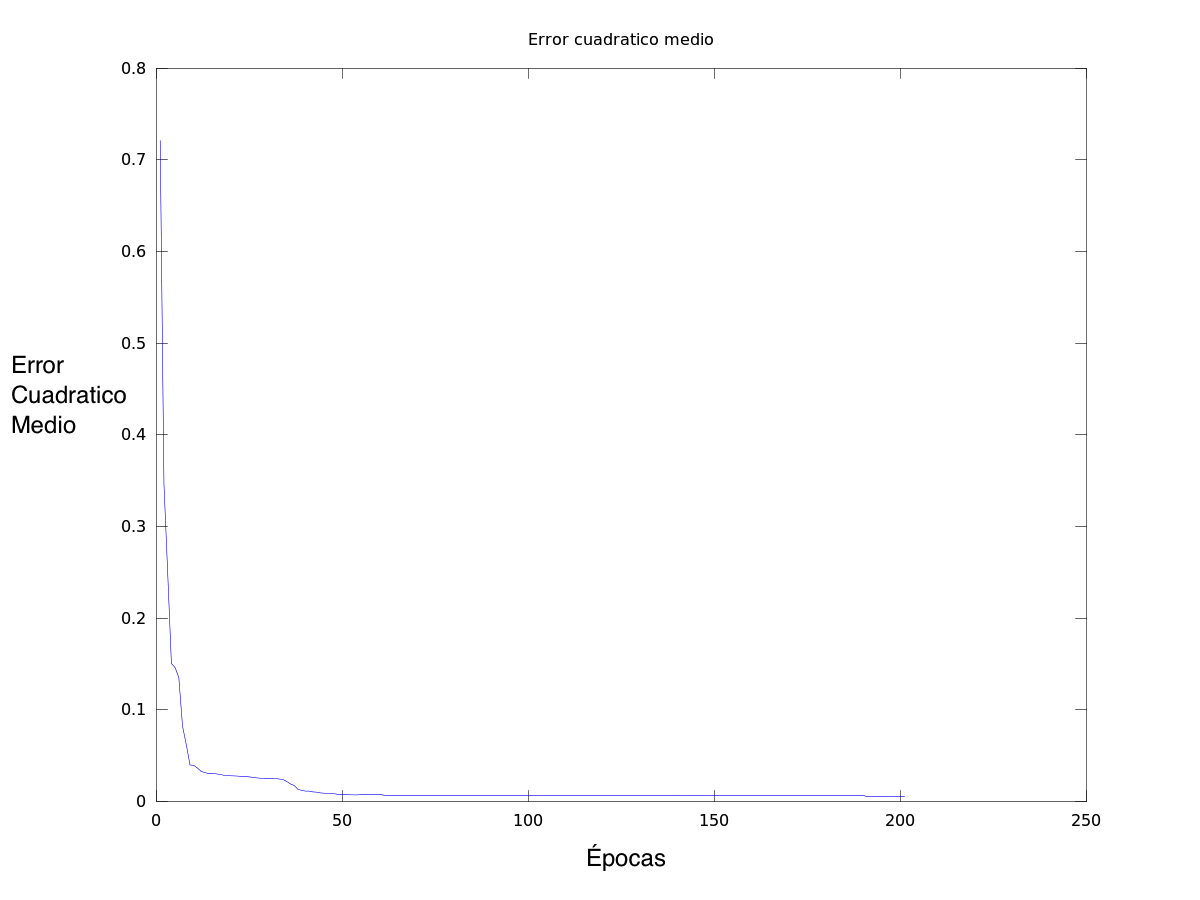
\includegraphics[scale=0.20]{images/t2-14/ecm.png}
\label{modelado}
\end{center}
\end{figure}
\end{frame}
\begin{frame}{Tercera Prueba}
\begin{figure}[H]
\begin{center}
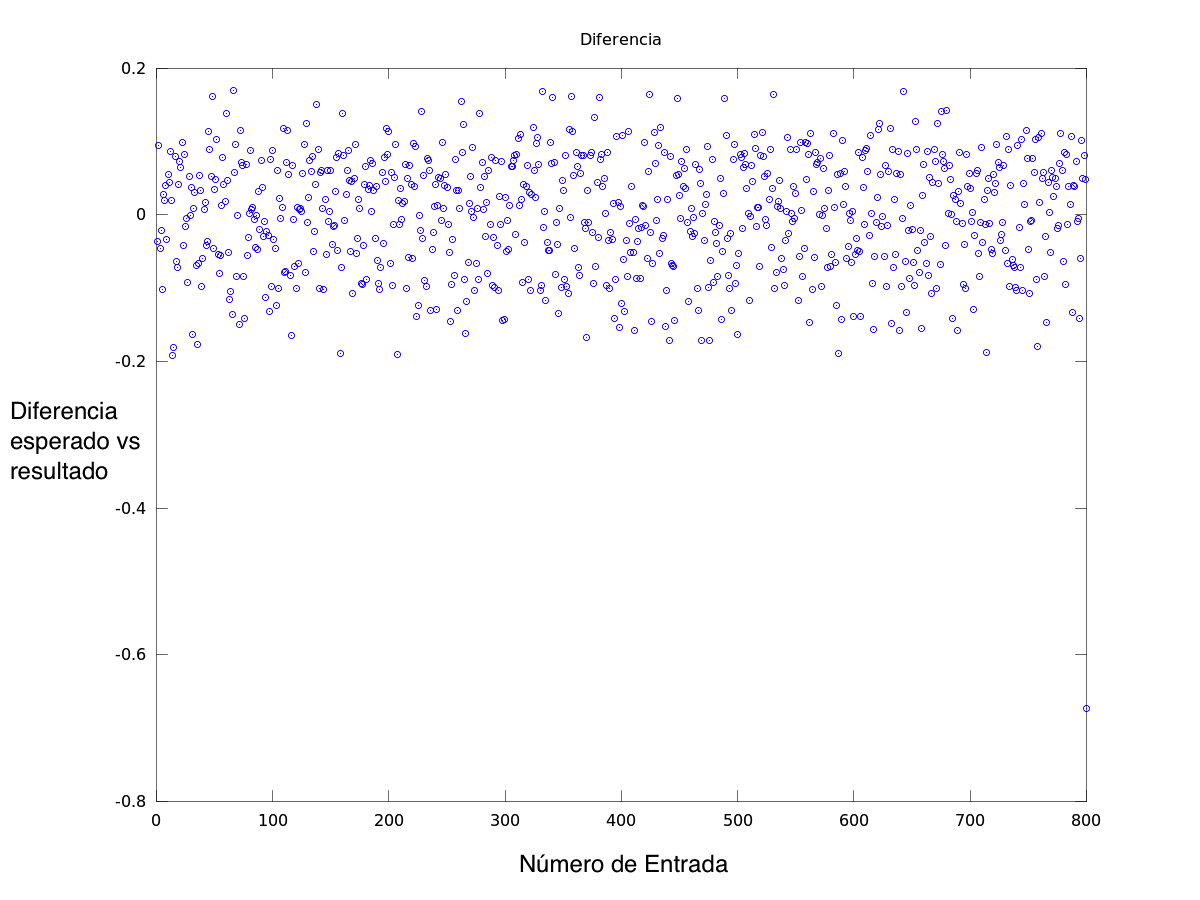
\includegraphics[scale=0.20]{images/t2-14/diferencia_final.png}
\label{modelado}
\end{center}
\end{figure}
\end{frame}


\section{Conclusiones}
\begin{frame}{Conclusiones}

\begin{itemize}
\item Incrementar la cantidad de neuronas no necesariamente 
implica mejoras en cuanto al error.
\item Los parametros dependen del problema que se esta resolviendo y su correcta elección es de gran importancia.
\item Activar el momentum no siempre acelera la convergencia.
\item Es posible aprender más aumentando el tamaño del conjunto de entrenamiento.
\end{itemize}

\end{frame}

\end{document}
